\subsection{Comparación entre las implementaciones en C y en ASM}
La primer parte de la experimentación consiste en realizar una comparación de performance de cada filtro en C (compilado con el nivel de optimización O3) con su contraparte en ASM (que aprovecha el modelo SIMD). A tal fin, en el caso del \emph{blur} sólo consideraremos la versión de control. Un análisis de performance de las versiones experimentales se realizará con posterioridad en la sección (\ref{subsec:resultados2}). Para que la comparación resulte lo más justa posible, tratamos de que a grandes rasgos los algoritmos en C y ASM no difieran demasiado, de tal forma que el uso de instrucciones SIMD (en el algoritmo de assembler) sólo implique un incremento de la cantidad de píxeles procesados por ciclo pero no una diferencia en el método con el que son tratados.

En primer término, plantearemos nuestras hipótesis con respecto a lo que esperamos que pase, y a continuación realizaremos un análisis de los resultados experimentales.

\subsubsection*{Hipótesis}
\paragraph*{Diferencia de imágenes}
Es importante destacar que, en términos de complejidad temporal, como el algoritmo escencialmente es el mismo en ambas implementaciones, al usar SIMD solo esperamos mejorar la constante pero no el orden de la complejidad. Dado que en la versión ASM estamos operando con cuatro píxeles en cada iteración, mientras que en C sólo lo hacemos de a uno, es esperable que la primer implementación sea poco menos de cuatro veces más rápida que la segunda. El ``poco menos''  hace referencia a que al usar SIMD necesitamos realizar algunas operaciones adicionales en ciertos casos; por ejemplo para hallar la máxima componente de los píxeles, hay que llamar dos veces a la función que calcula el máximo y realizar dos shifteos. En este sentido, también hay que considerar que la optimización de nivel O3 es muy agresiva. 

Otra cosa que esperamos que ocurra, es que el tiempo de procesamiento dependa sólo del tamaño de la imagen y no de otras características como los valores efectivos de los píxeles, pues en ningún momento los utilizamos para alterar el flujo del programa. Tampoco debería afectar que la imagen sea cuadrada o rectangular, si tienen la misma cantidad de píxeles en total.


\paragraph*{Blur gaussiano}
Las mismas hipótesis planteadas para la diferencia de imágenes valen para el blur, con la salvedad de que en este caso no procesamos de a cuatro píxeles por ciclo sino de a dos, con lo cual el procesamiento se espera sea un poco menos de dos veces más rápido. Adicionalmente, es fácil darse cuenta que al aumentar el radio que se pasa como parámetro aumenta también el tiempo necesario para procesar la imagen, pues la cantidad de iteraciones al calcular la convolución se incrementa. Puede ser interesante ver como varía la performance de cada implementación al aumentar el radio para un sigma fijo. En principio, se esperaría que los dos varíen de la misma forma.

\subsubsection*{Experimentos}
Los experimentos realizados para corroborar o rechazar nuestras hipótesis fueron los siguiente:
\begin{enumerate}
	\item Para el filtro \emph{diff}: 
		\begin{enumerate}
			\item \label{itm:exp-diff} Escogimos 11 tamaños de imagen distintos, generamos dos imágenes pseudo-aleatorias (con \emph{seeds} 100 y 142) de cada tamaño y luego corrimos 20000 iteraciones del filtro para cada par de imágenes de igual dimensión, primero con la implementación en C y luego con la de assembler.
		\end{enumerate}
	\item Para el filtro \emph{blur}:
		\begin{enumerate}
			\item \label{itm:exp-blur1}Análogo al experimento \ref{itm:exp-diff}, con 7 tamaños de imagen, y usando $\sigma=3$ y $radio=9$. \footnote{La cantidad de iteraciones usadas para realizar los experimentos fue variable en el caso de blur, pues como la cantidad de operaciones que realiza es alta y crece muy rápido con el tamaño de la imagen, los \emph{outliers} disminuyen significativamente con el mismo, pues el tiempo de cómputo adicional generado por cambios de contexto del sistema se ve amortizado, así como el efecto generado por mayores o menores \emph{hit-rates}. Esta aclaración vale para todos los experimentos sobre \emph{blur} de ahora en más.}
			\item Repetimos \ref{itm:exp-blur1} pero con $radio = 1$ y $\sigma = 0.3$ (el valor del $\sigma$ realmente es anecdótico pues en lo único que afecta es en el valor de los coeficientes del \emph{kernel}). El propósito de esto es comparar y explicar las diferencias con respecto al caso $radio = 9$.
			\item Fijadas las dimensiones de una imagen en 256x256, aplicamos \emph{blur} variando el radio.
		\end{enumerate}
\end{enumerate}

\subsubsection*{Resultados y análisis}
En la figura \ref{fig:exp.diff} podemos apreciar que como habíamos supuesto  

\begin{figure}
 	\centering
 	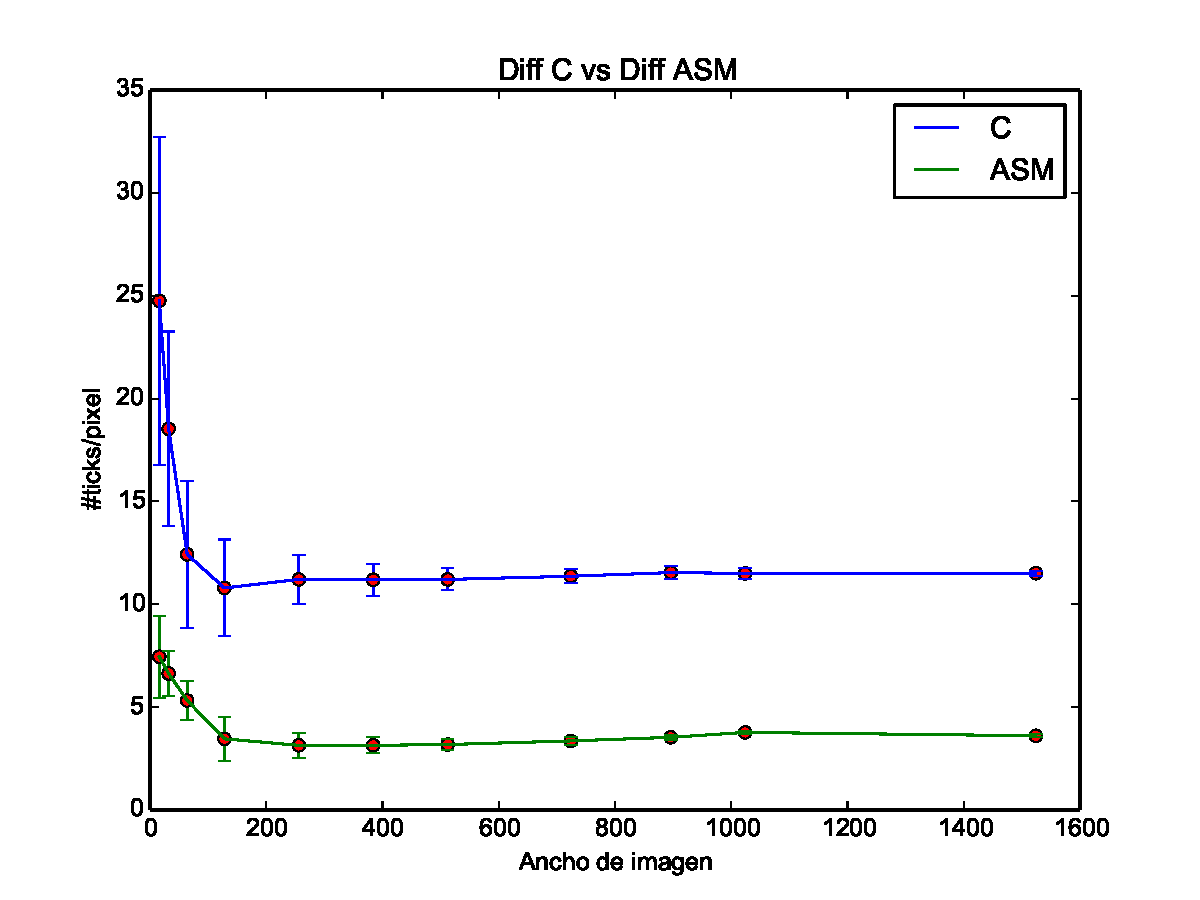
\includegraphics[width=0.75\textwidth]{../graficos/diff_gcc.pdf}
	\caption{\footnotesize Gráfico que muestra la cantidad de ticks de reloj por pixel que se requieren para aplicar el filtro de diferencias implementado en C y en assembler en función del ancho de la imagen. Todas las imágenes son cuadradas y fueron generadas pseudo-aleatoriamente. Los puntos rojos representan la media 0.25-podada calculada sobre las muestras obtenidas, mientras que los segmentos verticales indican la desviación standard.}
	\label{fig:exp.diff}
\end{figure}

\begin{figure}
 	\centering
 	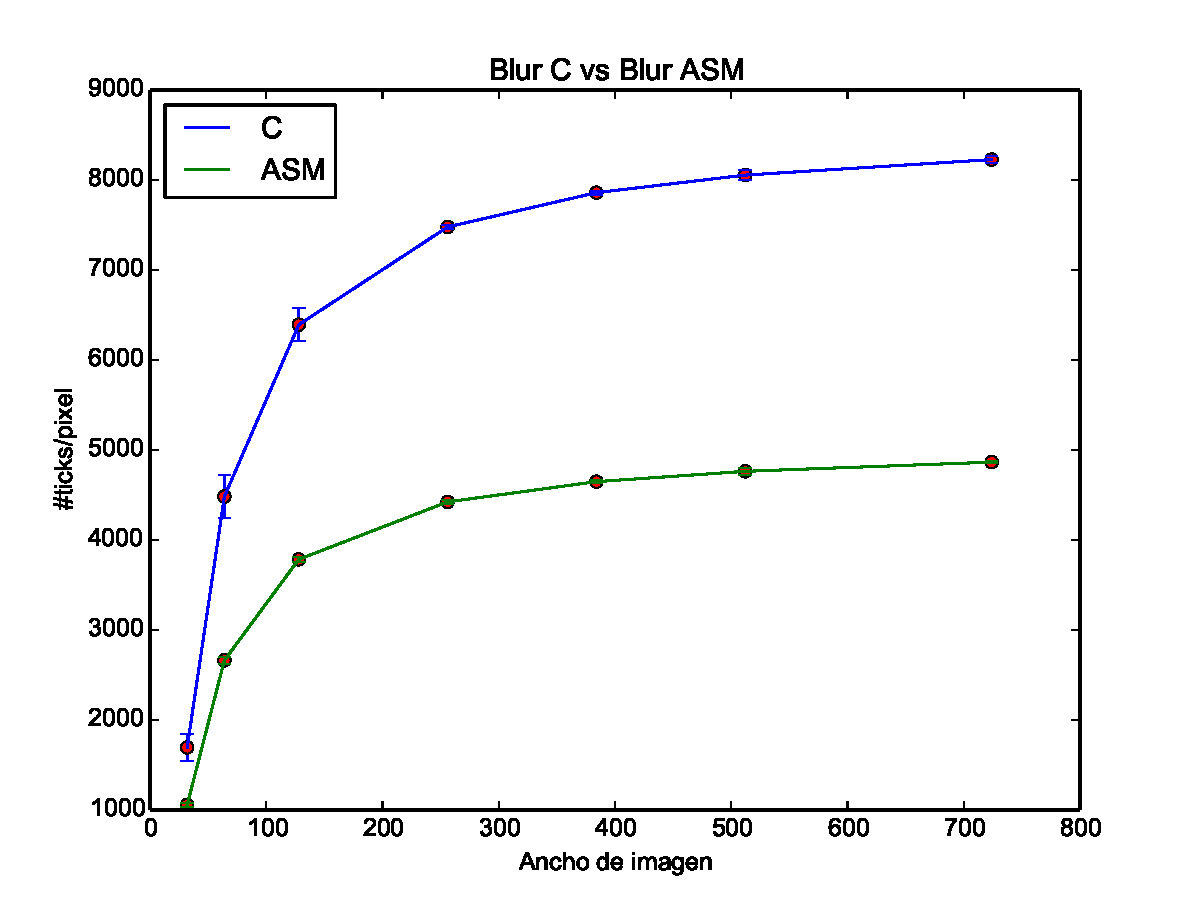
\includegraphics[width=0.75\textwidth]{../graficos/blur_v2_lineplot_3-9.pdf}
	\caption{\footnotesize Gráfico que muestra la cantidad de ticks de reloj por pixel que se requieren para aplicar el filtro de blur gaussiano implementado en C y en assembler en función del ancho de la imagen, para $\sigma = 3$, $radio = 9$ Todas las imágenes son cuadradas y fueron generadas pseudo-aleatoriamente. Los puntos rojos representan la media 0.25-podada calculada sobre las muestras obtenidas, mientras que los segmentos verticales indican la desviación standard.}
	\label{fig:lineplot.diff}
\end{figure}

\begin{figure}
 	\centering
 	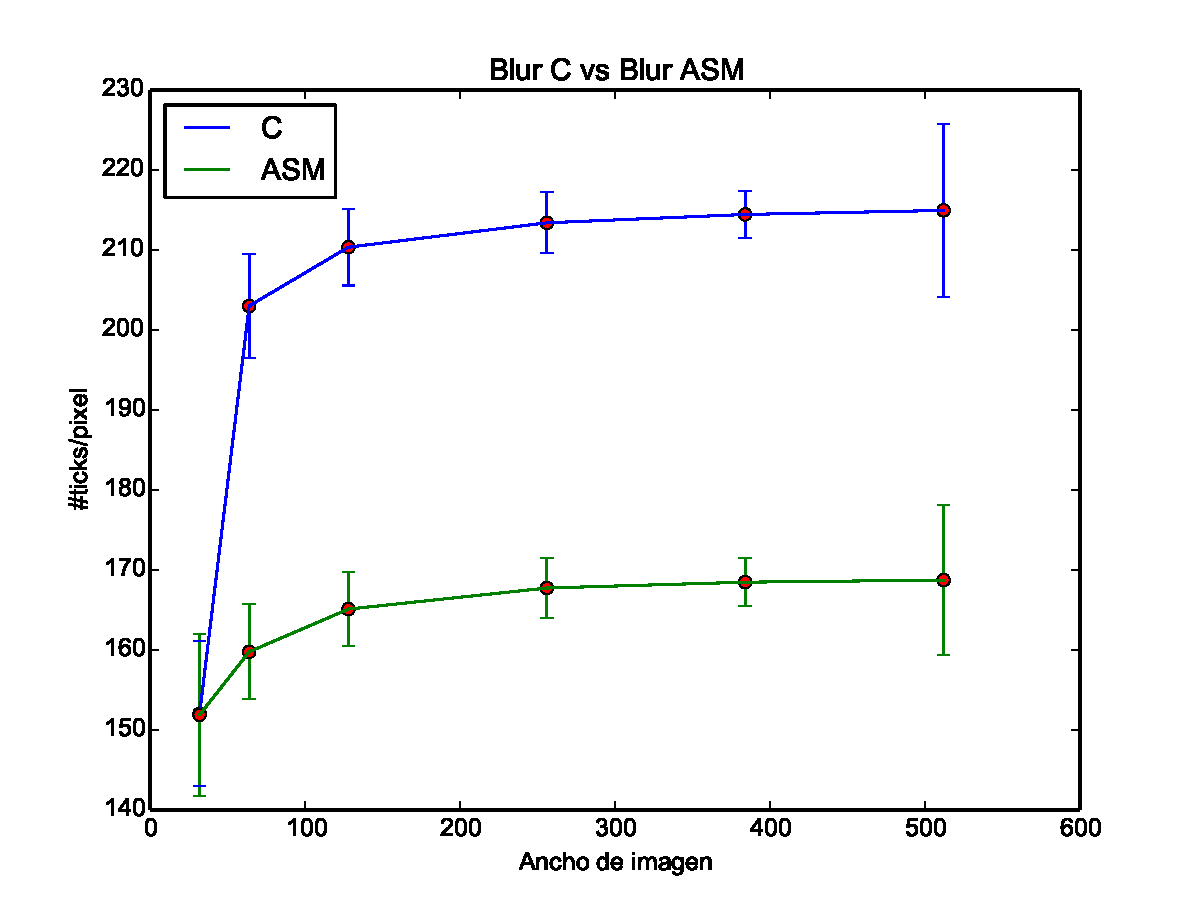
\includegraphics[width=0.75\textwidth]{../graficos/blur_v2_lineplot_0.3-1.pdf}
	\caption{\footnotesize Gráfico que muestra la cantidad de ticks de reloj por pixel que se requieren para aplicar el filtro de blur gaussiano implementado en C y en assembler en función del ancho de la imagen, para $\sigma = 3$, $radio = 9$ Todas las imágenes son cuadradas y fueron generadas pseudo-aleatoriamente. Los puntos rojos representan la media 0.25-podada calculada sobre las muestras obtenidas, mientras que los segmentos verticales indican la desviación standard.}
	\label{fig:lineplot.diff}
\end{figure}



%Posibles experimentos:
% *Para blur: fijar el sigma, y hacer un lineplot en función del radio